%
% Tesi D.S.I. - modello preso da
% Stanford University PhD thesis style -- modifications to the report style
%
%%%%%%%%%%%%%%%%%%%%%%%%%%%%%%%%%%%%%%%%%%%%%%%%%%%%%%%%%%%%%%%%%%%%%%%%%%%
%                                                                         %
%			TESI DOTTORATO                                                      %
%			______________                                                      %
%                                                                         %
%			AUTORE: Elena Pagani                                                %
%                                                                         %
%			                                                                    %
%                                                                         %
%%%%%%%%%%%%%%%%%%%%%%%%%%%%%%%%%%%%%%%%%%%%%%%%%%%%%%%%%%%%%%%%%%%%%%%%%%%
%
%
\documentclass[12pt]{report}
%    \renewcommand{\baselinestretch}{1.6}      % interline spacing
%
% \includeonly{}
%
%			PREAMBOLO
%
\usepackage[a4paper]{geometry}
\usepackage{amssymb,amsmath,amsthm}
\usepackage{mathtools}
\usepackage{fixltx2e}
\usepackage{graphicx}
\usepackage{subcaption}
\usepackage{url}
\usepackage{hyperref}
\usepackage{epsfig}
\usepackage[italian]{babel}
\usepackage{tesi}

% per le accentate
\usepackage[utf8]{inputenc}
%
\newtheorem{myteor}{Teorema}[section]
%
\newenvironment{teor}{\begin{myteor}\sl}{\end{myteor}}
%
%
%			TITOLO
%
\begin{document}
\title{PROFILE MATCHING IN ONLINE SOCIAL NETWORKS}
\author{Mattia Dimauro}
\dept{Corso di Laurea in Informatica per la Comunicazione}
\anno{2013-2014}
\matricola{808902}
\relatore{Prof. Sabrina GAITO}
\correlatore{Dr. Matteo Zignani}
%
%        \submitdate{month year in which submitted to GPO}
%		- date LaTeX'd if omitted
%	\copyrightyear{year degree conferred (next year if submitted in Dec.)}
%		- year LaTeX'd (or next year, in December) if omitted
%	\copyrighttrue or \copyrightfalse
%		- produce or don't produce a copyright page (false by default)
%	\figurespagetrue or \figurespagefalse
%		- produce or don't produce a List of Figures page
%		  (false by default)
%	\tablespagetrue or \tablespagefalse
%		- produce or don't produce a List of Tables page
%		  (false by default)
%
%			DEDICA
%
\beforepreface
\prefacesection{}
        {\hfill \Large {\sl dedicato a \dots}}
%
%			PREFAZIONE
%
\prefacesection{Prefazione}
Prefazione lalala.
%
%
%			ORGANIZZAZIONE
\section*{Organizzazione della tesi}
\label{organizzazione}
La tesi \`e organizzata come segue:
\begin{itemize}
\item nel Capitolo 1 ....
\end{itemize}
%
%			RINGRAZIAMENTI
%
\prefacesection{Ringraziamenti}
Ringrazio, grazie.
\afterpreface
%
%
%			CAPITOLO 1: Introduzione
\chapter{Introduzione}
\label{cap1}
Ciao volevo bla bla lba

%
%
\chapter{Pattern comportamentali e costruzione di features}
\label{cap2}
Gli individui mostrano spesso pattern comportamentali nella scelta dei loro usernames. Questi pattern, risultanti in ridondanza di informazione, possono essere utili per identificare individui su diversi social networks.
I soggetti potrebbero evitare queste ridondanze selezionando usernames in modo che risultino completamente diversi dai loro altri usernames. In questa maniera gli usernames risulterebbero essere talmente differenti che dato uno username, nessuna informazione riguardante gli altri usernames potrebbe essere estratta.
Idealmente per raggiungere questo stato di indipendenza tra usernames, l'individuo dovrebbe scegliere uno username che presenti entropia massima. Ovvero uno username composto da una lunga sequenza di caratteri, lunga quanto il massimo consentito dal sistema, senza ridondanze: una sequenza di caratteri completamente casuale.
Sfortunatamente, tutti questi requisiti non vengono incontro alle abilità umane. Gli esseri umani hanno difficoltà a memorizzare lunghe sequenze, con la possibilità della memoria a breve termine di ricordare 7$\pm$2 elementi. Queste limitazioni risultano condurre gli individui a selezionare generlamente usernames \textit{non lunghi}, \textit{non casuali} e che presentano \textit{abbondante ridondanza}.
Queste proprietà possono essere catturate adottando features specifiche.

Possiamo suddividere questi pattern comportamentali in tre categorie:
\begin{enumerate}
  \item Pattern dovuti a limitazioni umane
  \item Fattori esogeni
  \item Fattori endogeni
\end{enumerate}

Discuteremo dei comportamenti di ognuna di queste categorie elencate e delle features che possono essere estrapolate sfruttando questi pattern.


\section{Pattern dovuti a limitazioni umane}

\paragraph{definizione notazione}
Ci riferiremo a Individuo, username, prior usernames, candidate username.

\paragraph{Username identici}
Uno studio condotto da Zafarani dimostra che il 59\% degli individui preferisce usare lo stesso username reiteratamente, principalmente per facilitá nel ricordarlo.[citazione]

Quindi se un candidate username \textit{c} compare tra i prior usernames \textit{U}, vi é una forte indicazione che che potrebbe essere associato allo stesso individuo a cui sono associati i prior usernames. Considereremo dunque di utilizzare il numero di candidate username presenti tra i prior usernames come feature.

\paragraph{Username Length Likelihood}
Allo stesso modo, gli utenti hanno tipicamente un insieme di potenziali usernames dal quale ne estraggono uno quando richiesto di crearne uno nuovo. Questi usernames hanno differenti lunghezze e dunque é possibile calcolarne una distribuzione. Consideriamo \textit{l\textsubscript{c}} la lunghezza del candidate username e \textit{l\textsubscript{u}} la lunghezza di uno username \textit{u} $\in$ \textit{U}.
Assumiamo che per ogni nuovo username deciso di creare é probabile il verificarsi di\\
\centerline{$\min$\textit{l\textsubscript{u}} $\leq$ \textit{l\textsubscript{c}} $\leq$ $\max$\textit{l}\textsubscript{u}}
Ad esempio se un individuo é solito a scegliere username di lunghezza 8 o 9 caratteri, é improbabile che questo consideri di crearne uno con lunghezze minori o maggiori.
Considereremo quindi le lunghezza del candidate username e la distribuzione delle lunghezze dei prior usernames come features. La distribuzione verrá rappresentata da un numero fisso di features, descrivendola come\\
\centerline{($\mathbb{E}$[\textit{l\textsubscript{u}}],$\sigma$[\textit{l\textsubscript{u}}], med[\textit{l\textsubscript{u}}],$\min$\textit{l\textsubscript{u}},$\max$\textit{l\textsubscript{u}})}

\paragraph{Unique username creation Likelihood}

\paragraph{Limited Vocabulary}

\paragraph{Limited Alphabet}


\section{Fattori esogeni}
\section{Fattori endogeni}

%
%
\chapter{Collezione dataset}
\label{cap3}

Esistono più modalità attraverso le quali è possibile collezionare dati riguardanti stessi individui presenti su diversi social networks. Un modo semplice consisterebbe nel organizzare un questionario dove si richiede agli utenti di elencare i propri profili. Questo metodo permette di raccogliere una quantità di dati spesso limitata. Esistono compagnie, alcune risultano essere gli stessi social networks, che richiedono queste informazioni ai propri utenti ma queste non sono disponibili pubblicamente.
Fortunatamente esistono servizi di \textit{social network aggregation} che permettono di collezionare contenuti da diversi \textit{social network services} in una presentazione unificata. Il compito svolto da un \textit{social network aggregator}, che raggruppa insieme informazioni in un singolo luogo, supporta i propri utenti a riunire molteplici profili di social network in un singolo profilo e aiuta a tenere traccia delle attività che avvengono sui diversi profili semplificando la \textit{social networking experience} dell'utente.
La maggior parte di questi servizi non permette l'accesso pubblico alle informazioni aggregate, sono per lo più uno strumento per l'utilizzatore per seguire i propri profili, permettendo di avere tutte le notifiche relative in unico luogo, o di pubblicare lo stesso contenuto in più profili in una volta sola.Questa tipologia di aggregatori non sono frutto di interesse per la collezione di informazioni che cerchiamo.
Prenderemo in considerazione invece quegli aggregatori che permettono di condividere queste informazioni aggregate con altre persone. Attraverso questi è possibile visualizzare tutte le attività di un utente sui diversi social network che questo a deciso di far seguire all'aggregatore. Ovviamene è possibile, ed è l'informazione che andremo a estrarre, risalire su quale social network è stata eseguita tale azione e avere cosi un elenco di profili di social network services appartenenti alla stessa persona.
\section{Scraping Alternion}
\textit{Alternion - All your social web and email in one place -} è un aggregatore i cui servizi e features lo fanno rientrare tra la seconda classe di \textit{social network aggregator} descritta. Attraverso \textit{Alternion} è in fatti possibile per un utente condividere con altri contatti le informazioni riguardanti i propri profili di diversi online social networks. Il numero di utenti iscritti al servizio non è noto. Alternion dichiara di permettere ai propri utenti di aggregare un grosso numero di online social networks, dai più popolari come \textit{Facebook}, \textit{Twitter}, \textit{Google+}, \textit{LinkedIn}, \textit{Flickr} fino a più di 220 online social networks.
Di seguito spiegheremo l'approccio utilizzato al fine di ottenere i profili degli utenti iscritti al servizio e di recuperare da questi le informazioni riguardati i profili dei loro social networks. Alternion non dispone di un servizio per recuperare i dati attraverso un'interfaccia \textit{web (API)}, con richieste e risposte documentate. Dovremo dunque procedere analizzando le pagine web restituite svolgendo un'attività conosciuta come \textit{web scraping}.
Il \textit{web scraping} o \textit{web data extraction} è una tecnica di estrazioni di dati da pagine web. L'estrazione di dati viene automatizzata attraverso un software che simula un utente umano nell'esplorazione di documenti presenti sulla rete internet. Il software deve quindi implementare il protocollo HTTP, fondamento per la comunicazione di dati per il World Wide Web per recuperare il documento attraverso la rete internet. Questi documenti, tipicamente descritti attraverso un linguaggio di markup, sono pensati per rappresentare un'interfaccia grafica per l'utente. Ottenuto il documento il \textit{web scraper} si occupa di analizzarne i dati strutturati ricercandone quelli di interesse. La pagina non viene interpretata visivamente ma esaminandone il contenuto descritto con il linguaggio di markup, tipicamente HTML. Questa ricerca può essere effettuata con diversi approcci: dal più semplice, seppur potente, \textit{text grepping} combinato con \textit{regular expression matching} o può prevedere un'analisi più strutturata della pagina attraverso una tecnica di \textit{DOM parsing}. Per i nostri scopi utilizzeremo entrambe queste tecniche. Esistono altre tecniche e metodologie per eseguire \textit{web scraping}, ma i dettagli esulano dallo scopo di questa tesi.
\subsection{Ottenere i profili}
Siamo interessanti a ottenere un considerevole numero di profili di utenti che utilizzano l'aggregatore in analisi. Alternion non prevede una funzionalità per mostrare l'elenco completo dei profili iscritti al proprio servizio. Permette invece di reperirne un sotto insieme di questo attraverso una funzionalità di ricerca, divisibile in due classi: la ricerca parametrizzabile secondo alcuni criteri o la presentazione casuale di profili. La prima permette di interrogare il sistema per estrarne i profili corrispondenti ad alcuni parametri di ricerca come Nome, Sesso, Età, Paese di provenienza, Educazione, Interessi, etc La seconda funzionalità consente di ottenere ad ogni richiesta un profilo selezionato casualmente.\footnote{Più probabilmente, pseudo-casualmente!} Ho deciso di accantonare questa seconda via per due ragioni. La selezione casuale potrebbe potenzialmente portare a richiedere più volte lo stesso profilo, dipendentemente dalla bontà (che non è stata testata) della casualità con cui il profilo viene estratto. Vogliamo inoltre limitare l'estrazione di profili non appartenenti a persone fisiche: alcuni profili presenti fanno infatti riferimento a prodotti o società e aziende. Concludo di optare per la ricerca parametrizzata, in particolare, la ricerca per nome. Come lista di parametri per l'interrogazione del sistema useremo una lista di nomi propri \footnote{Lista reperita da census.gov}, formata da 4275 nomi femminili e 1219 maschili. Utilizzando strumenti messi a disposizione da Google\footnote{Google Chrome DevTools} per analizzarne i pacchetti HTTP scambiati tra il server di Alternion e il client Google Chrome, viene identificata la richiesta HTTP da eseguire per interrogare il server per farsi restituire la pagina web contenente la lista di utenti corrispondenti al parametro di ricerca. Eseguiremo quindi una richiesta per ogni nome presente nelle nostre liste di nomi. Da questa, tramite tecniche di scraping descritte precedentemente, estrapoliamo per ogni utente l'\textit{URL} idendificativo della risorsa. Una volta collezionati tutti gli URL, dove ogni indirizzo corrisponde a un utente di Alternion, potremo recuperare la pagina profilo di questi utenti e cercare al suo interno le informazioni riguardanti i loro social networks. Per la persistenza dei dati useremo MongoDB, un database NoSQL document-oriented, che utilizza JSON come data model.
\subsection{Profili recuperati}
Sono stati recuperati 15341 profili di Alternion, di cui 11274 presentano almeno due profili di social networks. Il numero di profili non è ingente, in quanto la funzionalità ricerca permette di recuperare un massimo di 30 profili per richiesta, ad esempio solo trenta profili delle persone che si chiamano `Anna'. Ad ogni modo si è notato che è possibile scalare, se non verticalmente per numero di users, orizzontalmente per numero di profili per users. Ogni utente ha in media $\sim$4,6 OSNS collegati, distribuiti tra un totale di 168 online social network services diversi presenti. Possiamo dunque espandere il numero di coppie di usernames secondo una combinazione semplice di \textit{n} elementi di classe \textit{k}, dove \textit{n} = 2 (coppie) e \textit{k} il numero di classi di OSN distinti. Ad esempio, un profilo \textit{P} ha aggreagato 3 OSNs \{Facebook, Twitter, Instagram \} e presenta quindi uno username \textit{u} per ogni profilo
\textit{U} = \{u\textsubscript{Alternion}, u\textsubscript{Facebook}, u\textsubscript{Twitter}, u\textsubscript{Instagram}\}. I sottoinsiemi di cardinalità 2 dell'insieme \textit{U} sono:
\begin{itemize}
  \item \{u\textsubscript{Alternion}, u\textsubscript{Facebook}\}
  \item \{u\textsubscript{Alternion}, u\textsubscript{Twitter}\}
  \item \{u\textsubscript{Alternion}, u\textsubscript{Instagram}\}
  \item \{u\textsubscript{Facebook}, u\textsubscript{Twitter}\}
  \item \{u\textsubscript{Facebook}, u\textsubscript{Instagram}\}
  \item \{u\textsubscript{Twitter}, u\textsubscript{Instagram}\}
\end{itemize}
Potenzialmente, il numero di classi di coppie di social network possibile é dimostrato essere uguale al coefficiente binomiale
\begin{gather*}
  \binom nk = \frac{n(n-1)\ldots(n-k+1)}{k(k-1)\dots1}
\end{gather*}
che puó essere scritto usando il fattoriale come
\begin{gather*}
  \frac{n!}{k!(n-k)!}
\end{gather*}
dove \textit{k} = 2 (coppie) e \textit{n} = 168, quindi 14028 coppie di social network distinte. Solamente 5855 di queste peró presentano almeno una coppia di username al suo interno. Concludendo, applicando la combinazione a 2 elementi per ogni profilo nel nostro dataset, otteniamo $\sim$170000 coppie di usernames. Con una media di $\sim$29 coppie di username per classe.
\paragraph{OSNS presenti}
\{100zakladokru, 43 Things, 500px, ActiveRain, All Consuming, Alternion, Amazon, Ameba, Aminus3, Answerbag, Aol Answers, AudioBoo, Bambuser, Bebo, Blipfm, Blipfoto, Bliptv, Blog Talk Radio, Blogger, Blogmarks, Blogru, Blogs@MailRu, Bordom, BuzzFeed, Buzznet, CafeMom, CiteULike, Connotea, Current, DailyStrength, Dailymotion, Delicious, DeviantART, Diigo, Disqus, Docstoc, Douban, Dreamwidth, Dribbble, EmpoweHER, Etsy, Eventbrite, FFFFound!, Facebook, Fancy, Flickr, FoodFeed, Formspring, Fotolog, Foursquare, FunnyOrDie, GamerDNA, Gamespot, Gather, GitHub, Gizmodo, Goodreads, Google Reader, Google+, Habrahabr, Hatena Bookmark, Hatena Diary, Hatena Haiku, HubPages, Hyves, Identica, Imgly, Instagram, Instructables, IntenseDebate, Ipernity, Issuu, Jalbum, JamBase, Judy"s Book, Lafango, Lastfm, LibraryThing, LinkedIn, Listal, Lookbooknu, Magma, MeasuredUp, Memoriru, Meneame, MetaFilter, Metacafe, Mister Wong, Moblog, MobyPicture, Multiply, Netlog, News2ru, Newsvine, NowPublic, Pandora, Panoramio, Photobucket, Photocase, Photosightru, Picasa, Pikchur, Pinboard, Pinterest, Plancast, Plixi, Plurk, Polyvore, Posterous, Qik, Qype, RPodru, Raptr, RedBubble, RedGage, Reddit, Rooftop Comedy, SAPO Fotos, SAPO Videos, Server Fault, Six Groups,Skyrock, SlideShare, SmugMug, Soupio, SparkPeople, Squidoo, Stack Overflow, StumbleUpon, Super User, Tabulas, Technorati, ThisNext, Threadless, TravelPod, Trilulilu, Tripit, Trulia, Tumblr, Tvigleru, Twitgoo, Twitpic, Twitrpix, Twitter, UserVoice, Viddler, VideoQip, Vimeo, Wattv, We Heart It, WordPress, Worth1000, Xanga, Yahoo! Answers, YouTube, Zazzle, Zenfolio, Zillow, Zorpia, aNobii, authorSTREAM, Facebook, gdgt, I use this, iPadio, iReport, Visualizeus, wePapers\}

\subsection{Distribuzione similaritá usernames}
Siamo interessati a confrontare coppie di usernames, per tentare di ricollegarle alla stessa entitá. Il caso piú semplice che potrebbe presentarsi\footnote{se non si considerano i casi di omonimia} é la corrispondenza esatta tra i due usernames. Indagheremo quindi questa proprietá sul nostro dataset acquisito. Oltre a verificarne la corrispondenza esatta, ovvero che le due stringhe che formano gli username presentino gli stessi caratteri nello stesso ordine, faremo uso di alcune metriche di similaritá su stringhe. Queste sono tecniche per quantificare la dissimilaritá tra due stringhe. In particolare utilizzeremo la \textit{distanza di Levensthein}, una metrica per misurare la differenza tra due sequenze, e \textit{l'indice di Jaccard}, un indice statistico utilizzato per comparare la similaritá e la diversitá di insiemi campionari.

\paragraph{Distanze}
Riportiamo le statistiche su le distanze calcolate su le classi aventi almeno 1000 coppie di username (29 classi, con un totale di 56687 coppie di usernames ) e su i dati globali.
\newline

\begin{tabular}{ r|c|c| }
\multicolumn{1}{r}{}
 &  \multicolumn{1}{c}{Mean Levensthein distance}
 & \multicolumn{1}{c}{Mean Jaccard Index} \\
\cline{2-3}
Popular classes & 6.2295 & 0.3277\\
\cline{2-3}
All dataset & 5.8159 & 0.3685 \\
\cline{2-3}
\end{tabular}

\paragraph{Match Esatti} Qui riportiamo le statistiche su i match esatti, dove le distanze di Levensthein e l'indice di Jaccard assume il valore 0.
\newline

\begin{tabular}{ r|c|c| }
\multicolumn{1}{r}{}
 &  \multicolumn{1}{c}{Levensthein distance = 0}
 & \multicolumn{1}{c}{Jaccard Index = 0 } \\
\cline{2-3}
Popular classes & 31.79\% & 34.03\% \\
\cline{2-3}
All dataset & 27.80\% & 29.16\% \\
\cline{2-3}
\end{tabular}

\begin{figure}[bp!]
\centering
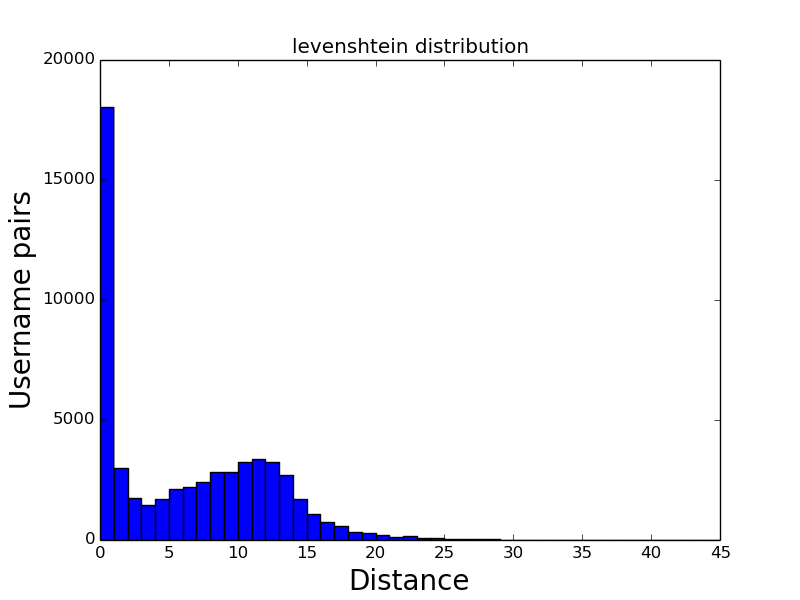
\includegraphics[width=110mm]{chapters/distanceplot/levenshtein_distribution.png}
\caption{Distribuzione distanza di Levensthein tra coppie di usernames  \label{overflow}}
\end{figure}

\begin{figure}[bp!]
\centering
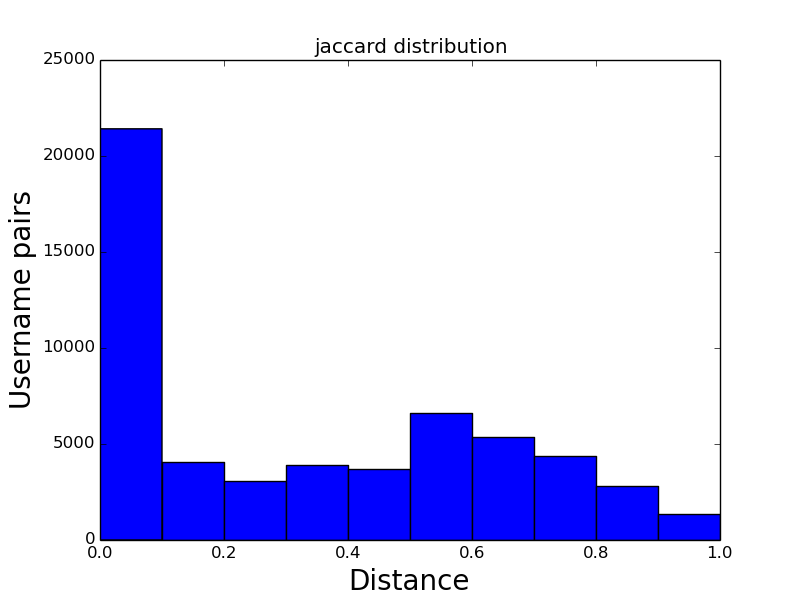
\includegraphics[width=110mm]{chapters/distanceplot/jaccard_distribution.png}
\caption{Distribuzione indice di Jaccard tra coppie di usernames \label{overflow}}
\end{figure}

\newpage

Osservando i dati rappresentati con un istogramma notiamo un pattern a \textit{doppio picco} che ritroviamo sia nel grafico delle distanze di Levensthein che dell'indice di Jaccard, su dati globali e anche analizzando classi prese singolarmente.


\begin{figure}
\begin{subfigure}{.5\textwidth}
  \centering
  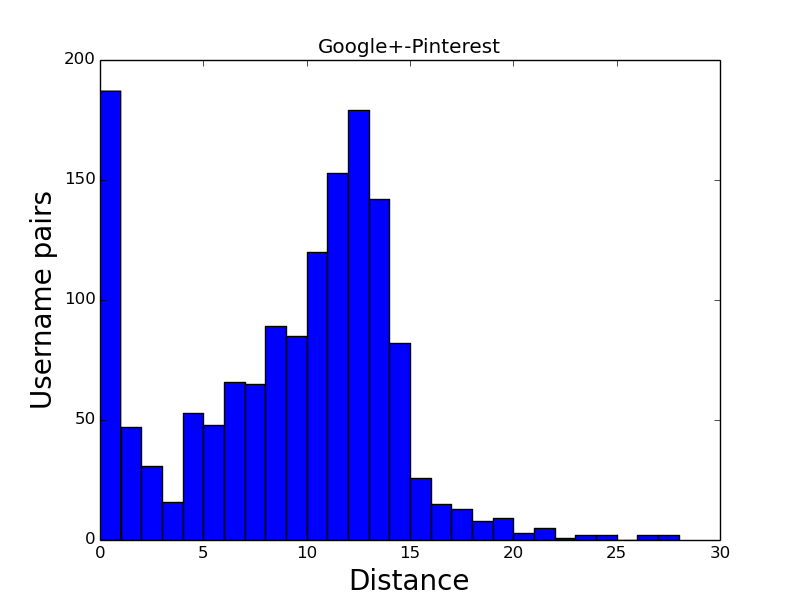
\includegraphics[width=.8\linewidth]{chapters/distanceplot/Google+-Pinterest.png}
  \caption{Google+ Pinterest}
  \label{fig:sfig1}
\end{subfigure}%
\begin{subfigure}{.5\textwidth}
  \centering
  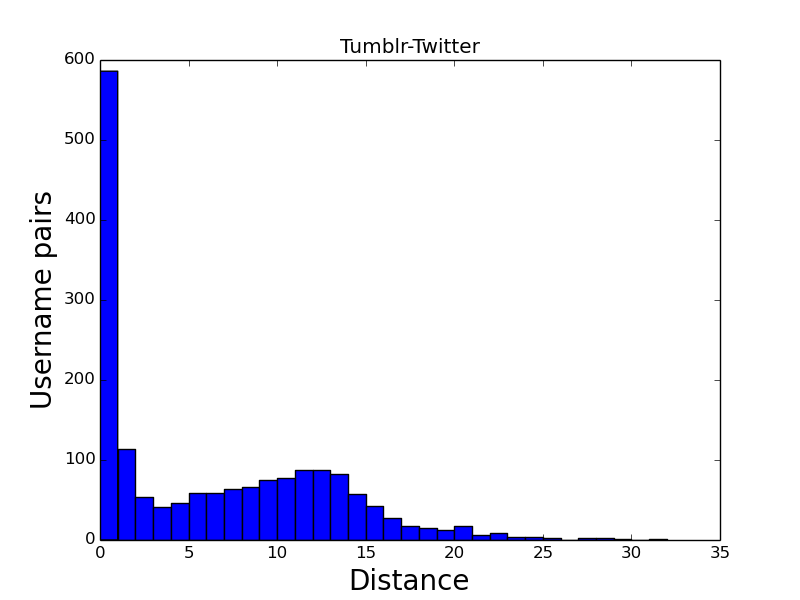
\includegraphics[width=.8\linewidth]{chapters/distanceplot/Tumblr-Twitter.png}
  \caption{Tumblr Twitter}
  \label{fig:sfig2}
\end{subfigure}
\caption{Pattern a doppio picco, anche su classe singola}
\label{fig:fig}
\end{figure}




Plottando le distanze di coppie di username casuali, non appartenenti alla stessa persona, ritroviamo invece una piú prevedibile distribuzione normale (Gaussiana).

\begin{figure}[bp!]
\centering
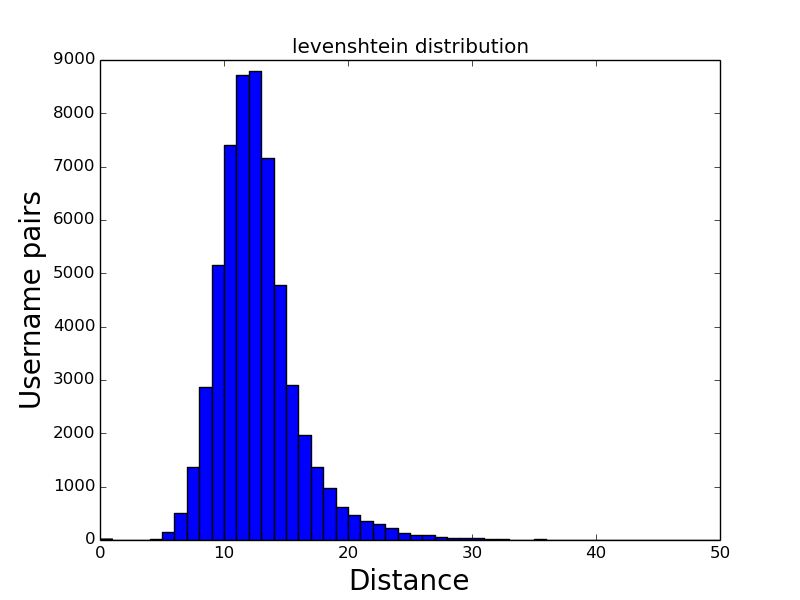
\includegraphics[width=110mm]{chapters/distanceplot/random_levenshtein_distribution.png}
\caption{Distribuzione distanza di Levensthein tra coppie random  \label{overflow}}
\end{figure}

\begin{figure}[bp!]
\centering
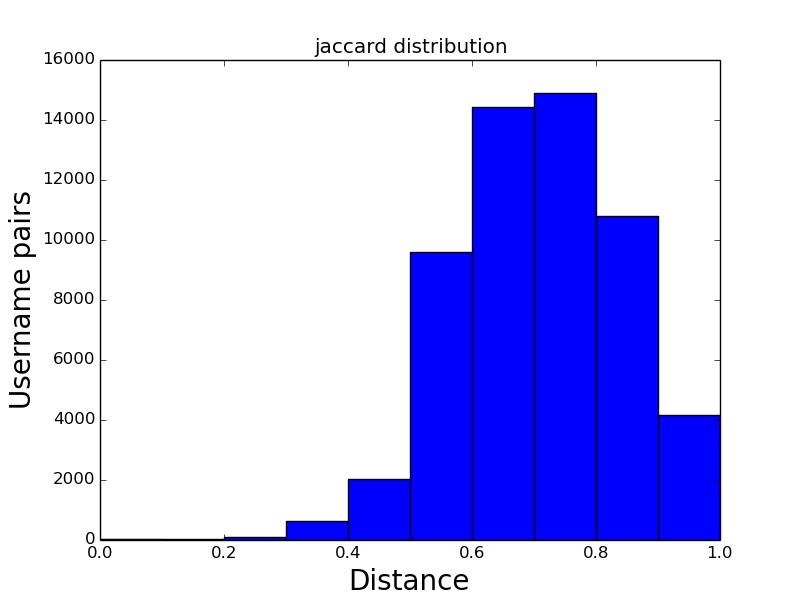
\includegraphics[width=110mm]{chapters/distanceplot/random_jaccard_distribution.png}
\caption{Distribuzione indice di Jaccard tra coppie random \label{overflow}}
\end{figure}

%
%
\chapter{Risultati}
\label{cap4}
Performance classificatore.


%
%			BIBLIOGRAFIA
%
\begin{thebibliography}{00}
%
\bibitem{gotti91}
M. Gotti, I linguaggi specialistici, Firenze, La Nuova Italia, 1991.
%
\bibitem{wellek62}
R. Wellek, A. Warren, Theory of Literature , 3rd edition, New York, Harcourt, 1962.
%
\bibitem{canziani78}
A. Canziani et al., Come comunica il teatro: dal testo alla scena. Milano, Il Formichiere, 1978.
%
\bibitem{MoD67}
Ministry of Defence, Great Britain, Author and Subject Catalogues of the Naval Library, London, Ministry of Defence, HMSO, 1967.
%
\bibitem{heine23}
H. Heine, Pensieri e ghiribizzi. A cura di A. Meozzi. Lanciano, Carabba, 1923.
%
\bibitem{basso62}
L. Basso, ``Capitalismo monopolistico e strategia operaia'', Problemi del socialismo, vol. 8, n. 5, pp. 585-612, 1962.
%
\bibitem{avirovic93}
L. Avirovic, J. Dodds (a cura di), Atti del Convegno internazionale "Umberto Eco, Claudio Magris. Autori e traduttori a confronto" ( Trieste, 27-28 novembre 1989), Udine, Campanotto, 1993.
%
\bibitem{gans67}
E.L. Gans, "The Discovery of Illusion: Flaubert's Early Works, 1835-1837", unpublished Ph.D. Dissertation, Johns Hopkins University, 1967.
%
\bibitem{harrison92}
R. Harrison, Bibliography of planned languages (excluding Esperanto).  \url{http://www.vor.nu/langlab/bibliog.html}, 1992, agg. 1997.
%
\end{thebibliography}
%
\end{document}
